
% !TEX TS-program = pdflatex
% !TEX encoding = UTF-8 Unicode

% This is a simple template for a LaTeX document using the "article" class.
% See "book", "report", "letter" for other types of document.

\documentclass[12pt, oneside, openany]{article} % use larger type; default would be 10pt

\usepackage[utf8]{inputenc} % set input encoding (not needed with XeLaTeX)

%%% Examples of Article customizations
% These packages are optional, depending whether you want the features they provide.
% See the LaTeX Companion or other references for full information.

%%% PAGE DIMENSIONS
\usepackage{geometry} % to change the page dimensions
\geometry{letterpaper} % or letterpaper (US) or a5paper or....
% \geometry{margin=2in} % for example, change the margins to 2 inches all round
% \geometry{landscape} % set up the page for landscape
%   read geometry.pdf for detailed page layout information

\usepackage{graphicx} % support the \includegraphics command and options

\usepackage[titletoc,toc,title]{appendix}

% \usepackage[parfill]{parskip} % Activate to begin paragraphs with an empty line rather than an indent

%%% PACKAGES
\usepackage{booktabs} % for much better looking tables
\usepackage{array} % for better arrays (eg matrices) in maths
\usepackage{paralist} % very flexible & customisable lists (eg. enumerate/itemize, etc.)
\usepackage{verbatim} % adds environment for commenting out blocks of text & for better verbatim
\usepackage{subfig} % make it possible to include more than one captioned figure/table in a single float
%\usepackage{forest} % Used for creating tree diagrams
\usepackage{color}
\usepackage{longtable}
\usepackage{amsmath}
% These packages are all incorporated in the memoir class to one degree or another...

%%% HEADERS & FOOTERS
\usepackage{fancyhdr} % This should be set AFTER setting up the page geometry
\pagestyle{fancy} % options: empty , plain , fancy
\renewcommand{\headrulewidth}{0pt} % customise the layout...
\lhead{}\chead{}\rhead{}
\lfoot{}\cfoot{\thepage}\rfoot{}

%%% SECTION TITLE APPEARANCE
\usepackage{sectsty}
%\allsectionsfont{\sffamily\mdseries\upshape} % (See the fntguide.pdf for font help)
% (This matches ConTeXt defaults)

%%% ToC (table of contents) APPEARANCE
\usepackage[nottoc,notlof,notlot]{tocbibind} % Put the bibliography in the ToC
\usepackage[titles,subfigure]{tocloft} % Alter the style of the Table of Contents
\renewcommand{\cftsecfont}{\rmfamily\mdseries\upshape}
\renewcommand{\cftsecpagefont}{\rmfamily\mdseries\upshape} % No bold!

\usepackage{listings}
%\usepackage{minted}

\newcommand{\deriv}[2]{\frac{\mathrm d #1}{\mathrm d #2}}
\newcommand{\pderiv}[2]{\frac{\partial #1}{\partial #2}}

%%% END Article customizations

\hyphenation{releaseNameAddressPhoneToThirdParty}

\begin{document}
\begin{titlepage}
\begin{center}
\vspace*{150px}
\LARGE{\textbf{An Examination of Networks in Computational Epidemiology} \\}
\vspace{12px}
\Large{Progress Report\\}
\vspace{12px}
\large{Anthony Culos, Zach Holland, and Emily Millard \\}
\vspace{12px}
\large{November 6th, 2015 \\}
\end{center}
\end{titlepage}
\tableofcontents
\newpage

\section{Introduction}

%%% Article Summary %%%
\section{Overview of \textit{Computational Epidemiology} as it Relates to our Project}
An epidemic can be characterized as a widespread occurrence of an illness or other health-related event at a particular time; a pandemic is an epidemic of worldwide proportions. Due to emerging global trends of increasingly dense urbanization, more local and global travel, and a generally older population, controlling and responding to future epidemics and possibly pandemics will become significantly more challenging. However, advances in computing, big data, and computational thinking have created new opportunities to control and prevent the spread of infectious disease. Computation plays a pivotal role in supporting real-time epidemiology because using controlled experiments to understand the spread of disease is much harder to perform than computer modeling, and often experiments are impossible due to ethical constraints. 

In 1760 Daniel Bernoulli developed the first mathematical model in epidemiology. Using his model, Bernoulli established that vaccination could help increase the life expectancy in the French population. Presently, the simplest and most commonly used model to demonstrate epidemic processes is the \emph{SIR} model. In this model a population of size $N$ is divided into three states: susceptible ($S$), infective ($I$), and removed or recovered ($R$). Each infected person can infect any susceptible person (independently) with probability $\beta$ and can recover with probability $\gamma$. Let $S(t)$, $I(t)$, and $R(t)$ represent the number of people that are in either the susceptible, infected, or removed states at a given time $t$. Furthermore let $s(t) = \frac{S(t)}{N}$, $i(t) = \frac{I(t)}{N}$, and $r(t) = \frac{R(t)}{N}$. (i.e. the fractions of the population in each of the states.) And it follows that: $s(t) + i(t) + r(t) = 1$. 

Using the complete mixing requirement which assumes that every person is in contact with everyone in the population, the following system of differential equations describe the dynamics of the SIR model:

\begin{align}
	\deriv{s(t)}{t} &= -\beta s(t) i(t) \\
	\deriv{i(t)}{t} &= \beta s(t) i(t) - \gamma i(t) \\
	\deriv{r(t)}{t} &= \gamma i(t)
\end{align}

A common use for the SIR model is to determine the likelihood of an epidemic infecting a large fraction of the population. According to the SIR model, a large scale infection will occur if and only if $R_{0} = \frac{\beta}{\gamma} > 0 $, where $R_{0}$ is the \textit{reproductive number}. Public health decision making is often very concerned with controlling $R_{0}$.

The SIR model makes many assumptions, the most significant of which is the complete mixing requirement which is often unrealistic. A more recent approach to understand the spread of an epidemic is \textit{networked epidemiology}. Networked epidemiology seeks to understand the interactions between three distinct components of epidemiology: individual behaviors of agents; unstructured, heterogeneous multi-scale networks; and the dynamical processes on these networks. This type of analysis is focused on the belief that a better understanding of the underlying network and individual behaviors within the network will provide better insights into contagion dynamics and response strategies. 

To apply this network model, let $G(V, E)$ denote a contact graph on a population, where $V$ is the set of people in the population and $E$ is the set of contact pairs in the population (i.e. $\{u,v\}\in E~ \mathrm{iff}~u,v\in V~\mathrm{and}~u,v$ have come into contact with each other). Additionally, let $N(v)$ denote a set of neighbors of $v$. Applying the SIR model to $G$, a node is in either a $S$, $I$, or $R$ state. For each $\{u,v\}$ pair, infection can potentially spread along edge $e = \{u, v\}$ with probability of $ \beta(e,t) $ at time $t$ after $u$ becomes infected. This probability is conditional on node $v$ remaining susceptible until time $t$.~\cite{marathe} 

\subsection{Technology Diffusion as an Analogue to Disease Transmission}
It has been well studied that the adoption of new ideas, norms, behaviors, and products through an interpersonal network closely resembles the spread of infectious disease through an affected population~\cite{goel}. Due to the difficulty of finding proper examples of population contact networks and their associated disease transmission networks, we propose to use interpersonal networks and the diffusion of technology adoption on those networks as an analogue.

%%% Data Analysed %%%
\section{Data Analysed}
We were able to find a comprehensive data set of information diffusion from ``The Anatomy of a Scientific Rumor'' by Domenico et al.~\cite{domenico}. They tracked the information spreading process across Twitter after the announcement of the the discovery of a particle displaying the properties of the Higgs boson on July 4th, 2012. The researchers made their data available through the Stanford Network Analysis Project (SNAP)~\cite{snap}, which is a repository of large network datasets. We analyzed two networks: the first being the contact network in which the information of the Higgs discovery spread, and the greater friends/followers network of all Twitter users involved in the information diffusion. The diffusion network has Twitter users as nodes, and interactions such as mentions, replies, and retweets as edges. Each edge represents a direction of infection between users. The larger contact network has users as nodes and the edges represent the relationship between the user and its direction (i.e. following, follower). It is important to note that a single interaction can incur multiple edges from a node. For instance if a user mentions another in a tweet that gets retweeted both a mention and a retweet edge will be produced going from the retweeting account to each other user respectively.

\section{General Diffusion Analysis}
\subsection{Strategy}
The diffusion information was analyzed in intervals of 300 seconds, instead of analyzing the diffusion over each second this made computation much easier as it reduced the amount of data points from 563069 to 2016. The diffusion analysis will consist of two different datasets constructed from the original data provided by SNAP. The first being the sum of all infection events over a given time interval and the amount of infected nodes at a given time interval, and the second being the sum of all infection events with respect to mentions, replies, and retweets. The analysis will be focused on the first dataset, and it will be compared to the second. We will then compare our results of the analysis to see whether it agrees with the literature of diffusion on large networks which states that large cascades are extremely rare, and if they occur the majority of infections occur within one degree of the seed~\cite{goel}. That is, we can expect to see a large infection event occur and then the and then the infection should very quickly die off.

\subsection{Analysis}
The most current literature of diffusion on large networks states that the network should be inactive until a large cascade of infections occurs. This cascade will start very quickly and will die out very soon after it started. Our analysis agrees with these findings, it is then important to look at the infections prior to and after the cascade. Information on the infections per time period are given by Table~\ref{tbl:stats}, and this information is visualized in figures~\ref{fig:infection-count},~\ref{fig:newly-infected}, and~\ref{fig:overlay}.

\begin{table}
\centering
\begin{tabular}{| c || c | c | c | c |}
	\hline
   		& Standard Dev. & Mean & Max & Variance \\
   	\hline\hline
  	New Infections & 544.785 & 278.301 & 4765 & 296643.668 \\
	\hline
\end{tabular}
  \caption{Some general statistics of the rates of infection for each time period.}
  \label{tbl:stats}
\end{table}

\begin{figure}
\centering
    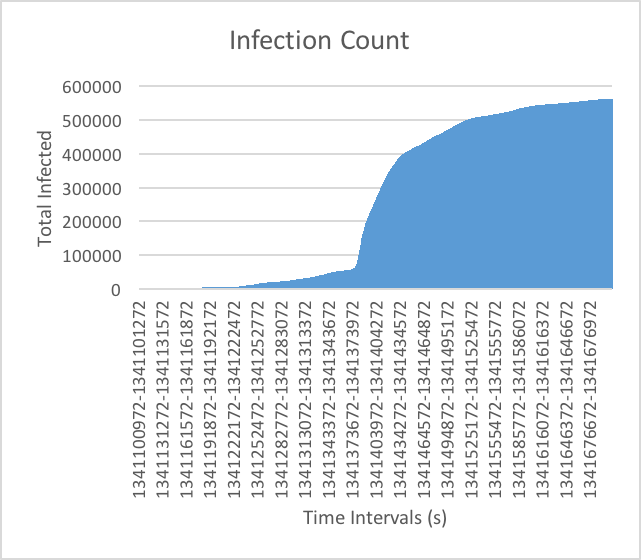
\includegraphics{infection-count.png}
    \caption{The cumulative number of infections for all the time intervals.}
    \label{fig:infection-count}
\end{figure}

\begin{figure}
\centering
    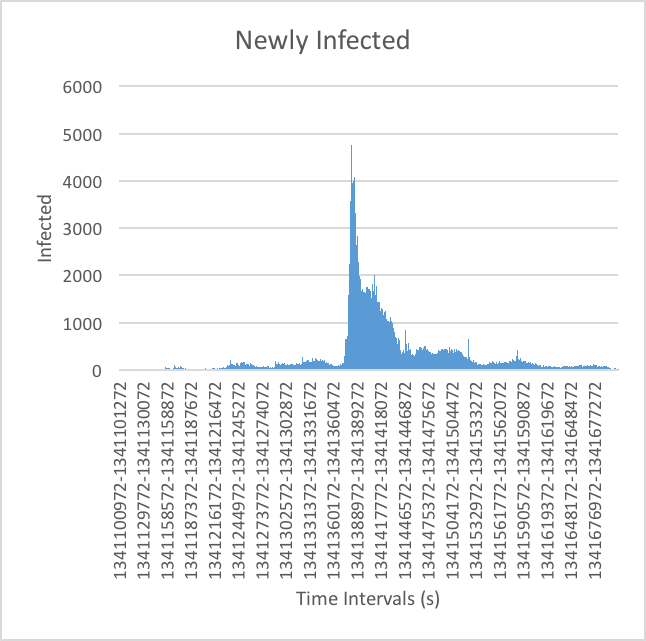
\includegraphics{newly-infected.png}
    \caption{The number of new infections during each time interval.}
    \label{fig:newly-infected}
\end{figure}

If we overlay the two plots from figures~\ref{fig:infection-count} and~\ref{fig:newly-infected} (as is shown in Figure~\ref{fig:overlay}) it becomes obvious that the majority of infections happens within a very short amount of time relative to the total time of the diffusion.

\begin{figure}
\centering
    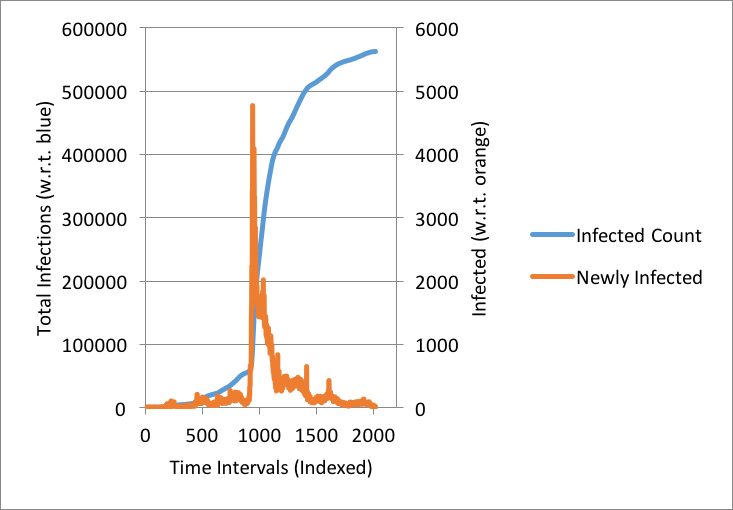
\includegraphics{overlay.png}
    \caption{The overlay of the two plots from figures~\ref{fig:infection-count} and~\ref{fig:newly-infected} shows the relation between number of new infections and the total number of infections at a given interval.}
    \label{fig:overlay}
\end{figure}

Between the times 1341380272-1341430372 (time since the UNIX Epoch in seconds) 298571 infections occur out of a total 563069 infections over the lifetime of the diffusion. This 835 min (approximately 14 hour) period accounts for over 50\% of all the infections. This agrees with our predictions that the information will both start and end quickly after the initial cascade event. The growth and decay of infections is even more evident if we split our data before and after the peak infection time as is shown in Figure~\ref{fig:before-after}.

\begin{figure}
\centering
    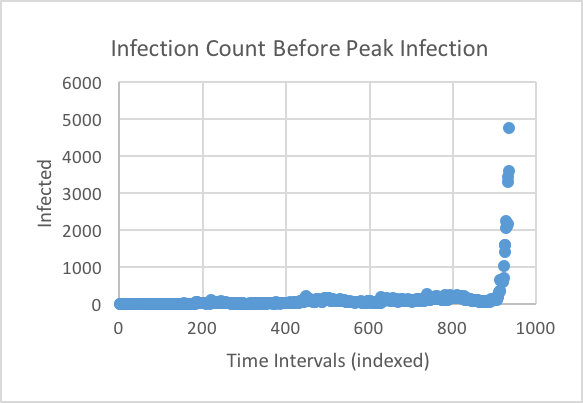
\includegraphics{before.png}
      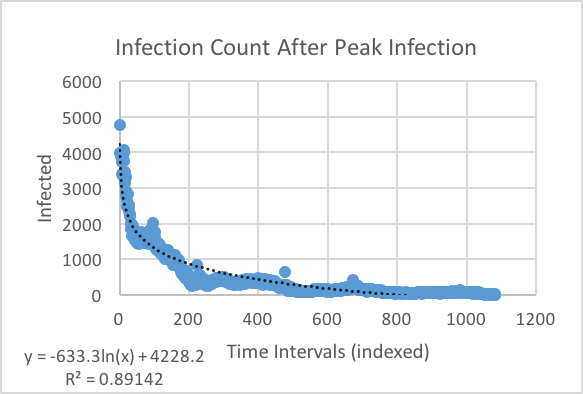
\includegraphics{after.png}
    \caption{Display the number of new infections before and after the peak infection. This shows very well how rapidly information diffuses and then decays on large networks.}
    \label{fig:before-after}
\end{figure}

Now that we have a general understanding of how the diffusion of the Higgs boson announcement spreads on a large network, we will now analyze the specific avenues of diffusion available (replies, mentions, and retweets) for any anomalies.

\begin{table}
\centering
\begin{tabular}{| c || c | c | c | c |}
	\hline
   		& Standard Dev. & Mean & Variance &Total \\
   	\hline\hline
  	Replies & 32.342 & 18.305 & 1045.999 & 36902 \\
  	\hline
  	Mentions & 152.613 & 84.939 & 23290.67 & 171237 \\
  	\hline
  	Retweets & 362.454 & 176.057 & 131373.1 & 354930 \\
	\hline
\end{tabular}
  \caption{Statistics of each type of diffusion observed in the SNAP Higgs boson data set.}
  \label{tbl:type-stats}
\end{table}

\begin{figure}
\centering
    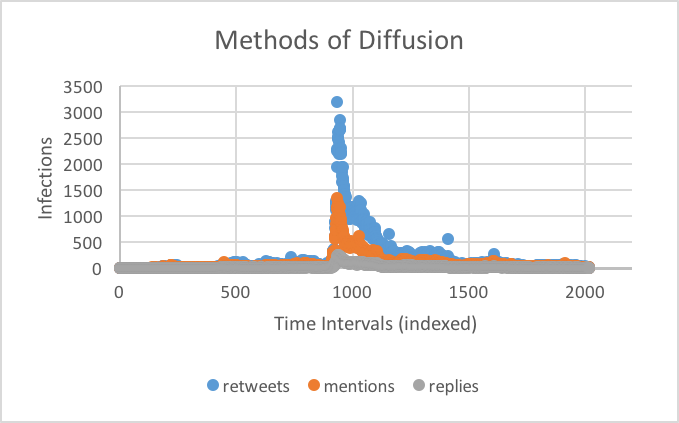
\includegraphics{methods.png}
    \caption{Shows how the different means of diffusion relate to each other.}
    \label{fig:methods}
\end{figure}

As Table~\ref{tbl:type-stats} and Figure~\ref{fig:methods} show the rate of infection of each method of diffusion, this follows closely to the aggregate diffusion data with no deviation from what we expect to see. It is interesting to note the popularity of the methods used to spread the Higgs announcement. The most popular method being the one with the least involvement (retweeting) and the most involved method of interaction (reply) is the least popular. This is most likely due to the majority of people not being motivated enough about the discovery to start a conversation but reach a minimum interest in the subject to want to spread the news.

\subsection{Conclusion}
We expect the information of the Higgs boson discovery to diffuse on this network in a similar fashion as other large networks. With little to no activity to begin with and then a large infection event that begins and decays at a very quick rate. Which would account for the majority of the infections during the lifetime of the diffusion. This is true for the infections in aggregate and the specific methods of infection observed in this network. All of these criteria are met so we can conclude that the discovery of the Higgs boson follows the expected behavior of diffusion.

\section{Diffusion Analysis In Terms of the Community Structure of the Contact Network}
\subsection{Community Structure of Networks}
\subsection{Diffusion Through Communities}
\subsection{Conclusion}

\newpage
\begin{thebibliography}{1}
 \bibitem{marathe} 
 M. Marathe and A. Vullikanti. ``Computational Epidemiology.'' \emph{Communications of the ACM}, vol. 56, no. 7, pp. 88-96, 2013.
 \bibitem{goel} 
 S. Goel \emph{et al}. ``The Structure of Online Diffusion Networks,'' in \emph{Proceedings of the 13th ACM Conference on Electronic Commerce}. New York, NY: ACM. 2012. pp. 623-638.
 \bibitem{domenico}
 D. Domenico \emph{et al}. ``The Anatomy of a Scientific Rumor.'' \emph{Scientific Reports}, vol. 3, no. 2980. Oct. 18, 2013.
\bibitem{snap}
Stanford Network Analysis Project. ``Higgs Twitter Dataset,'' Accessed Nov. 2015, https://snap.stanford.edu/data/higgs-twitter.html
 \end{thebibliography}

\end{document}